\documentclass[varwidth=20cm]{standalone}

\usepackage{tikz}
\usetikzlibrary{positioning,arrows}
\usepackage[european]{circuitikz}
\usepackage{pgfplots}
\pgfplotsset{compat=1.18}

% This file contains configuration shared between main file and figures

\usepackage{pifont}
\usepackage{xspace}
\DeclareUnicodeCharacter{2460}{\ding{172}\xspace}
\DeclareUnicodeCharacter{2461}{\ding{173}\xspace}

\usepackage{tikz}

\definecolor{HB9UFblue}{RGB}{0,61,165}
\definecolor{HB9UFred}{HTML}{ED135A}

\newcommand{\Ohm}{$\Omega$\xspace}


\newcommand{\uline}[1]{%
  \tikz[baseline=(todotted.base)]{
      \node[inner sep=1pt,outer sep=0pt] (todotted) {#1};
      \draw[color=HB9UFblue,thick] (todotted.south west) -- (todotted.south east);
  }%
}%
                           
\newcommand{\udash}[1]{%
  \tikz[baseline=(todotted.base)]{
      \node[inner sep=1pt,outer sep=0pt] (todotted) {#1};
      \draw[dashed,color=HB9UFred,thick] (todotted.south west) -- (todotted.south east);
  }%
}%


\begin{document}
    \begin{circuitikz}
        \draw (0,0) to[sinusoidal voltage source=$U_Q$] (0,-4)
              (0,0) to[short] (3,0) to[R,a=50~$\Omega$] (3,-2) to[short,-o] (5,-2)
              (3,-2) to[R,a=50~$\Omega$,*-*] (3,-4) to[short,-o] (5,-4)
              (3,-4) to[short,-*] (0,-4) node[ground] {};
        \draw[-stealth',shorten >=3mm,shorten <=3mm] (5,-2) -- node[right]{$U_L$} (5,-4);
     \end{circuitikz}
    \hspace{5mm}
    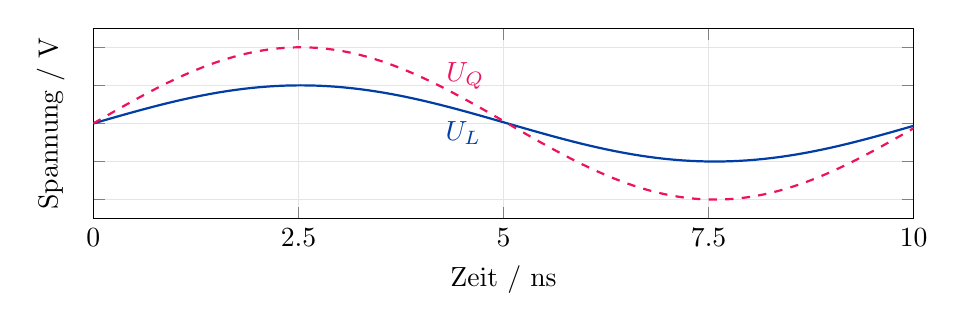
\begin{tikzpicture}
        \begin{axis}[
            xmin=0, xmax=10,
            ymin=-1.25,ymax=1.25,
            ylabel={Spannung / V},
            grid=both,
            xlabel={Zeit / ns},
            yticklabels={},
            xtick = {0,2.5,5,7.5,10},
            ytick = {-1,-0.5,0,0.5,1},
            height=4cm,
            width=12cm,
            major grid style={black!10}
        ]
        \addplot [mark=none,samples=100,domain=0:10,color=HB9UFblue,thick] {0.5*sin(3600*x)} node[below,pos=0.45] {$U_L$};
        \addplot [mark=none,samples=100,domain=0:10,color=HB9UFred,dashed,thick] {sin(3600*x)} node[above,pos=0.45] {$U_Q$};;
        \end{axis}
    \end{tikzpicture}

    \vspace{5mm}

    \begin{circuitikz}
        \draw (0,0) to[sinusoidal voltage source=$U_Q$] (0,-4)
              (0,0) to[short] (3,0) to[R,a=50~$\Omega$] (3,-2) to[short,-o] (5,-2)
              (3,-2) to[L,a=80~nH,*-*] (3,-4) to[short,-o] (5,-4)
              (3,-4) to[short,-*] (0,-4) node[ground] {};
        \draw[-stealth',shorten >=3mm,shorten <=3mm] (5,-2) -- node[right]{$U_L$} (5,-4);
    \end{circuitikz}
    \hspace{5mm}
    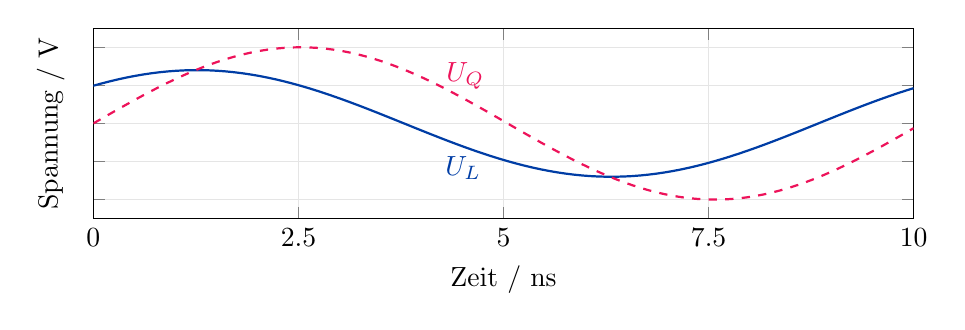
\begin{tikzpicture}
        \begin{axis}[
            xmin=0, xmax=10,
            ymin=-1.25,ymax=1.25,
            ylabel={Spannung / V},
            grid=both,
            xlabel={Zeit / ns},
            yticklabels={},
            xtick = {0,2.5,5,7.5,10},
            ytick = {-1,-0.5,0,0.5,1},
            height=4cm,
            width=12cm,
            major grid style={black!10}
        ]
        \addplot [mark=none,samples=100,domain=0:10,color=HB9UFblue,thick] {0.7*sin(3600*x+45)} node[below,pos=0.45] {$U_L$};
        \addplot [mark=none,samples=100,domain=0:10,color=HB9UFred,dashed,thick] {sin(3600*x)} node[above,pos=0.45] {$U_Q$};;
        \end{axis}
    \end{tikzpicture}
\end{document}
